


\subsection{Challenges}
Measuring the context switch time in serverless functions has several challenges:
\begin{itemize}
	\item [C1] Characteristics of context switch in serverless environments
	
	Context switch is triggered differently in serverless functions compared to in traditional operating systems as it's scheduled by the cloud provider.
	And the service provider has the tendency to trigger more functions in the same hardware to get more profits. 
	Thus, context switch may happen not only due to performance factors like multi-threading/processing, but also provider's profit considerations.
	
	\item [C2] Benchmark accuracy
	
	As none of the existing benchmarks can be used in serverless environment, 
	it's challenging for us to reason about the accuracy of new benchmarks proposed.
	We also have to reason about the potential factors that might lead to variations in the measurement.
%	As no such benchmark is provided so far, we have to analyze the factors in our own benchmark that may lead to the potential variation to golden value, 
%	in order to reason about the accuracy of the measurement.
	% Variations to golden values in measurement 
\end{itemize}

\subsection{Reasoning context switches in serverless environment}
	In a cloud setting, the cloud provider will allocate multiple users to share the same physical device, in order to maximize the computing resource utilization.
	When there are multiple users co-locating at the same server, if the number of processes needed to run is larger than the cores inside the server, it's highly likely that there will be context switches. 
	
	Figure\ref{fig:cloud} shows one example scenario. 
	
	







	To tackle \emph{C1}, we design the following experiments to analyze the factors influencing context switch in serverless environments.
	We measure the execution time elapse between two adjacent lines of code repeatedly under different configurations in serverless functions.
	Shahrad \emph{et al.} \cite{serverless-main} shows that the execution time in serverless functions is influenced by function invocation frequency, memory size and function execution time.
	Thus, these configurations will include the function invocation rate, memory allocated.
	Theoretically, the measured time elapse should be 0 as there is no execution between these two lines. 
	However, our initial experiments show that this is neither 0 nor a fixed value, indicating that interruption happens between these two lines
	and the time elapse changes with different configurations. 
	Although the interruption is not limited to context switch but also page faults handling or container management, 
	it can still provide insights in the influence of different configurations on context switch time in serverless environments.


\subsection{Combine various benchmarks}
	To tackle \emph{C2}, we first run our own designed benchmarks on local Linux system and compare the results with published benchmarks\cite{cs-lmbench,cs-pipes,cs-arm,cs-web},
	 ensuring the correctness of the proposed ones. Then we deploy the new benchmarks in serverless functions and compare the results. 
	 If one of the benchmarks is consistently higher or lower than others, then we'll explore the reasons and this can help us improve our accuracy.

	The previous benchmarks in context switching on Linux system mainly consider %some fa
	Our initial study to \emph{C1} finds that context switch in serverless environments will also be influenced by invocation rate and memory allocation.   

	Currently, the new benchmarks are designed as the prior benchmarks with different configurations.
	The prior benchmarks we are choosing are:
	
	1. Pingpong pipes\cite{cs-pipes,cs-web}: Two threads or processes are created. 
		      One thread/process writes the data to another process through a pipe, which induces a context switch. 
			  After the data is read, the read thread/process transfers the data to write thread/process and this induces another context switch.
			  The total execution time equals the read and write operation time adds two context switch time.
			  In contrast, a single process is created. It passes the data through a pipe to itself. 
			  Here the total execution time only consists of the read and write operation time.
			  By subtracting these two time and dividing the result with 2, we get the context switch time.
	
	2. Condition var\cite{cs-web}: A shared variable between two threads is used and is protected by mutex to prevent it from being modified by two threads at the same time.
		      A signal is passed between two threads to tell which thread has the access to write the variable.
			  And by passing the signals, the context will switch from one thread to the other. 
			  The time for the signal changes is the context switch time.
	
	3.  Lmbench\cite{cs-lmbench}: A ring of pipes is created, and a token is passed from process to process with these pipes. 
	          Also, the time of passing the token in a single process with this ring of pipes is measured. 
			  Subtraction of these two time is the total context switch time of a number of context switches.

	Next, we'll implement these functions with different invocation rate and memory allocation setting in the cloud,
	to measure the influence of configurations on the context switch time.
	
\begin{figure}
	\centering
	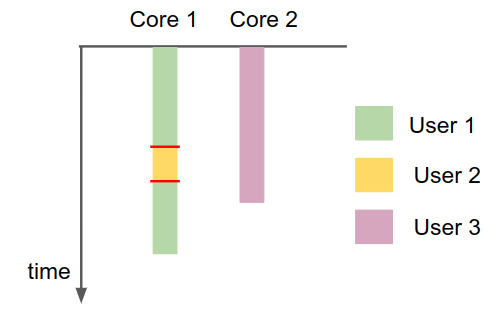
\includegraphics[width=\linewidth]{./figure/cxt_cloud.png}
	\caption{Context switches in serverless computing}
	\label{fig:cloud}
\end{figure}

% "Based on these traditional methods, we also used pipe communication to implement frequent context switches between two processes."
